% This file was created with tikzplotlib v0.10.1.post5.
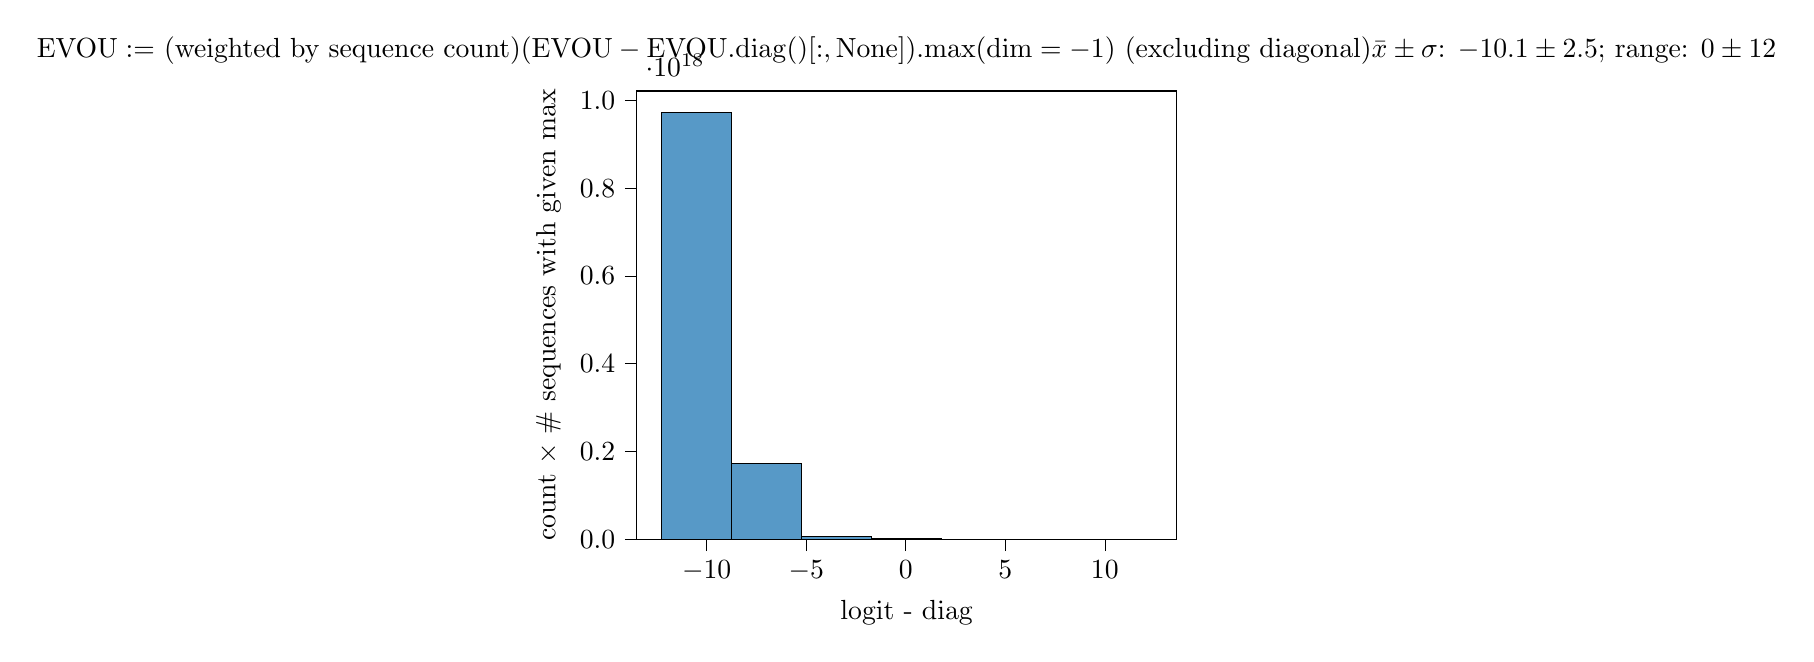
\begin{tikzpicture}

\definecolor{darkgray176}{RGB}{176,176,176}
\definecolor{steelblue31119180}{RGB}{31,119,180}

\begin{axis}[
tick align=outside,
tick pos=left,
title={\(\displaystyle \mathrm{EVOU} := \WE \WV \WO\WU \) (weighted by sequence count)\\
\(\displaystyle (\mathrm{EVOU} - \mathrm{EVOU}\mathrm{.diag}()[:,\mathrm{None}])\mathrm{.max}(\mathrm{dim}=-1)\) (excluding diagonal)\\
\(\displaystyle \bar{x}\pm\sigma\): \(\displaystyle -10.1 \pm 2.5\); range: \(\displaystyle 0 \pm 12\)},
x grid style={darkgray176},
xlabel={logit - diag},
xmin=-13.5117744922638, xmax=13.5995020389557,
xtick style={color=black},
xtick={-15,-10,-5,0,5,10,15},
xticklabels={
  \(\displaystyle {\ensuremath{-}15}\),
  \(\displaystyle {\ensuremath{-}10}\),
  \(\displaystyle {\ensuremath{-}5}\),
  \(\displaystyle {0}\),
  \(\displaystyle {5}\),
  \(\displaystyle {10}\),
  \(\displaystyle {15}\)
},
y grid style={darkgray176},
ylabel={count \ensuremath{\times} \# sequences with given max},
ymin=0, ymax=1.02139487497023e+18,
ytick style={color=black},
ytick={0,2e+17,4e+17,6e+17,8e+17,1e+18,1.2e+18},
yticklabels={
  \(\displaystyle {0.0}\),
  \(\displaystyle {0.2}\),
  \(\displaystyle {0.4}\),
  \(\displaystyle {0.6}\),
  \(\displaystyle {0.8}\),
  \(\displaystyle {1.0}\),
  \(\displaystyle {1.2}\)
}
]
\draw[draw=black,fill=steelblue31119180,fill opacity=0.75] (axis cs:-12.2794437408447,0) rectangle (axis cs:-8.75849873679025,9.72757023781167e+17);
\draw[draw=black,fill=steelblue31119180,fill opacity=0.75] (axis cs:-8.75849873679025,0) rectangle (axis cs:-5.23755373273577,1.72418997143109e+17);
\draw[draw=black,fill=steelblue31119180,fill opacity=0.75] (axis cs:-5.23755373273577,0) rectangle (axis cs:-1.71660872868129,5.68110592851047e+15);
\draw[draw=black,fill=steelblue31119180,fill opacity=0.75] (axis cs:-1.71660872868129,0) rectangle (axis cs:1.80433627537319,1.56419338866055e+15);
\draw[draw=black,fill=steelblue31119180,fill opacity=0.75] (axis cs:1.80433627537319,0) rectangle (axis cs:5.32528127942766,483504484421024);
\draw[draw=black,fill=steelblue31119180,fill opacity=0.75] (axis cs:5.32528127942766,0) rectangle (axis cs:8.84622628348214,981026585330);
\draw[draw=black,fill=steelblue31119180,fill opacity=0.75] (axis cs:8.84622628348214,0) rectangle (axis cs:12.3671712875366,15698854392871);
\end{axis}

\end{tikzpicture}
